\section{Linking}

\section{Virtual Memory}
All Assembly code is executed using virtual memory. At no point is it aware of the actual hardware address.

The MMU is in charge of converting these physical addresses to virtual ones, and vice-versa. This can lead to problems however with fragmentation.

    \subsection{Page Tables}
    \begin{figure}[ht]
        \centering
        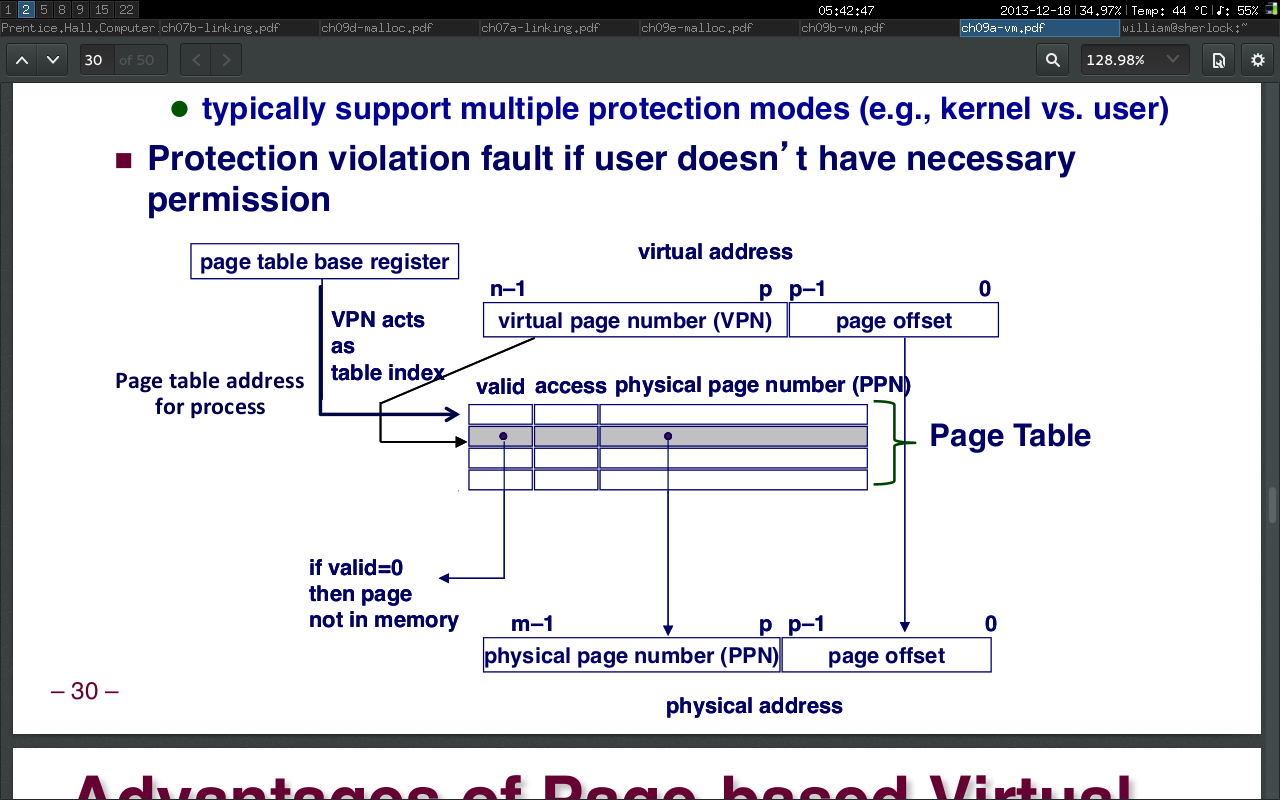
\includegraphics[scale=0.2]{./img/pagetable.png}
    \end{figure}

    To help solve this, most machines use fixed length pages, usually 4 KB. The virtual page number is equal to the virtual address divided by the size of the page.

    Page tables also map main memory to these fixed size pages as well. The page table records a virtual page $\to$ hardware page mapping.

    A page table is an array of page tables entries (PTE) that maps virtual pages to physical ones.

    The virtual address space, $\{0, 1, 2, \cdots, N-1\}$, with $N = 2^n$, is mapped to the physical address space, $\{0, 1, 2, 3, \cdots, M - 1\}$.

    Physical pages are $P=2^p$ bytes in size and have been partitioned into 3 disjoint subsets. Unallocated have not been create by the VM system. Cached are currently in memory. Unchached are not.

    There is a valid bit on each row that indicates whether or not the row is currently in memory.

    \begin{figure}[ht]
        \centering
        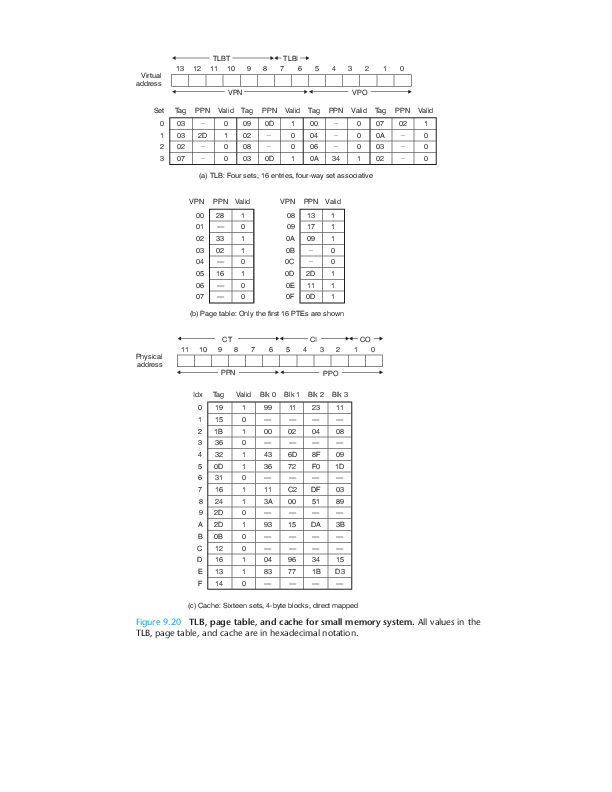
\includegraphics[scale=0.8]{./img/addresses.png}
    \end{figure}

    \begin{table}[ht]
        \centering
        \begin{tabular}{|l|l|}
            \hline
            \textit{Symbol} & \textit{Description}\\
            \hline
            \hline
            $N=2^n$ & Number of addresses in virtual space\\
            $M=2^m$ & Number of addressses in physical space\\
            $P=2^p$ & Page size (bytes)\\
            \hline
            VPO & Virtual page offset (bytes)\\
            VPN & Virtual page number\\
            TLBI & TLB index\\
            TLBT & TLB tag\\
            \hline
            PPO & Physical page offset\\
            PPN & Physical page number\\
            CO & Byte offset within cache block\\
            CI & Cache index\\
            CT & Cache tag\\
            \hline
        \end{tabular}
    \end{table}
